\section{Results}

\subsection{Telencephalon and optic tectum are sharply separated at the proteoform level}

The first substantive result of this paper is a new quantitative statement about adult zebrafish brain organization: the public top-down record places telencephalon and optic tectum in sharply distinct proteoform regimes. At the article level, telencephalon contributes 309 identified proteoforms and optic tectum contributes 533, but only 35 proteoforms are shared, yielding the published Jaccard overlap of 0.0434. The region-specific fractions are 0.8867 for telencephalon and 0.9343 for optic tectum. The released source tables tell the same story while making the evidence chain much tighter. Exact accession+proteoform matching across \texttt{Proteoform\_ID\_Tel2.xlsx} and \texttt{proteoform\_ID\_Teo2.xlsx} yields 29 shared entries over a union of 805, corresponding to an exact-ID Jaccard of 0.0360 and an exact-ID S{\o}rensen overlap of 0.0689. Using raw mean duplicate intensities barely changes the picture: the weighted Jaccard is 0.0427 and the Bray--Curtis similarity is 0.0820. Alternative normalizations stay in the same regime rather than rescuing a high-overlap interpretation. Per-run total-intensity scaling yields weighted Jaccard 0.0557 and Bray--Curtis 0.1055, upper-quartile scaling yields 0.0452 and 0.0864, and median-ratio scaling yields 0.0430 and 0.0824. Looking directly at the four duplicate run pairs reaches the same conclusion: raw run-pair weighted Jaccard spans 0.0192--0.0476 and raw run-pair Bray--Curtis spans 0.0377--0.0909, while the per-run-total-normalized pairwise values span 0.0200--0.0687 and 0.0393--0.1285. A 10{,}000-draw row bootstrap over the intensity tables gives a weighted-Jaccard median of 0.0212 (95\% interval 0.0030--0.0639) and a Bray--Curtis median of 0.0415 (0.0060--0.1201), again leaving the analysis in the same low-similarity regime. Even at the protein level, the overlap remains modest at 0.2151. A prevalence-adjusted lower-tail overlap test sharpens the same point. Relative to the fixed-margin independence baseline, the exact-ID centered Jaccard is $-0.2792$ and the lower-tail $p$ value is $5.56\times10^{-183}$; after collapsing to proteins, the centered Jaccard is still $-0.2130$ with $p = 5.84\times10^{-33}$. In other words, the public dataset does not describe two lightly shifted samples; it describes two strongly separated regional proteoform profiles, with the sharper separation only becoming visible once proteoforms are kept distinct.

The discrepancy between the article's 35 shared proteoforms and the table-derived exact-ID count of 29 is also diagnosable rather than mysterious. If bracketed PTM annotations and punctuation are stripped before matching while accessions are retained, the shared count rises to 44. Tightening that relaxed rule by also requiring residue-window agreement leaves the same shared count and almost the same Jaccard (0.0609 instead of 0.0615), and a residue-window-only match yields the same result again. The published value therefore sits between a strict exact-ID match and a small family of relaxed deterministic encodings, which is what one would expect if article-side aggregation used representation choices that are not fully documented in the PRIDE tables. The supplementary workbook's note sheet strengthens that reading because it states that the released tables were generated with 1\% PrSM FDR and 5\% proteoform-level FDR in TopPIC plus TopDiff duplicate quantification, making a pure table-side threshold mismatch a less attractive explanation than a representation or aggregation mismatch. The important point is that none of those choices turn the dataset into a high-overlap case.

The duplicate-resolved source tables also let us address the obvious undersampling objection more directly than before. The Tel2 table contains 154 singleton detections and 155 duplicate detections, yielding a Chao2 lower-bound richness of 385.5 proteoforms; the Teo2 table contains 355 singletons and 178 duplicate detections, yielding a Chao2 lower bound of 887.0 proteoforms. A first-order incidence jackknife gives a similar but slightly less extreme pair of lower bounds, 386.0 and 710.5. If the observed 29 shared exact IDs are held fixed while the Chao2 unseen richness is added, the overlap drops to a Jaccard of 0.0233. If instead the shared overlap is inflated by the smaller, geometric-mean, or larger of the region-specific duplicate-inflation factors, the Jaccard remains between 0.0293 and 0.0394. The jackknife fixed-shared scenario yields 0.0272. A 10{,}000-draw row-resampling sensitivity analysis pushes in the same direction rather than reopening the case: the median exact-ID Jaccard falls to 0.0227 with a 95\% interval of 0.0133--0.0326, the median canonicalized Jaccard is 0.0436 with interval 0.0308--0.0567, and the protein-collapsed overlap median is 0.1831 with interval 0.1528--0.2133. The reviewer's minimal MNAR-style alternative is also too small to rescue a high-overlap story: imputing missing exact IDs to half of the region-specific 5th-percentile or 10th-percentile nonzero intensity shifts weighted Jaccard only to 0.0456 and 0.0483, and Bray--Curtis only to 0.0873 and 0.0922. All of those values still sit in the same ``very low overlap'' regime as the original article-level value.

\begin{table}[t]
\centering
\caption{Core regional separation metrics supporting the regional-organization claim. The first two rows preserve the article-level summary, and the remaining overlap rows use the released exact-ID tables.}
\label{tab:summary}
\begin{tabular}{lr}
\toprule
Metric & Value \\
\midrule
Article shared proteoforms & 35 \\
Article Jaccard overlap & 0.0434 \\
Exact-ID shared proteoforms & 29 \\
Exact-ID Jaccard overlap & 0.0360 \\
Exact-ID S{\o}rensen overlap & 0.0689 \\
Weighted Jaccard overlap & 0.0427 \\
Bray--Curtis similarity & 0.0820 \\
Canonicalized shared proteoforms & 44 \\
Telencephalon unique fraction & 0.8867 \\
Optic tectum unique fraction & 0.9343 \\
Protein overlap fraction & 0.2151 \\
\bottomrule
\end{tabular}
\end{table}

\begin{figure}[t]
    \centering
    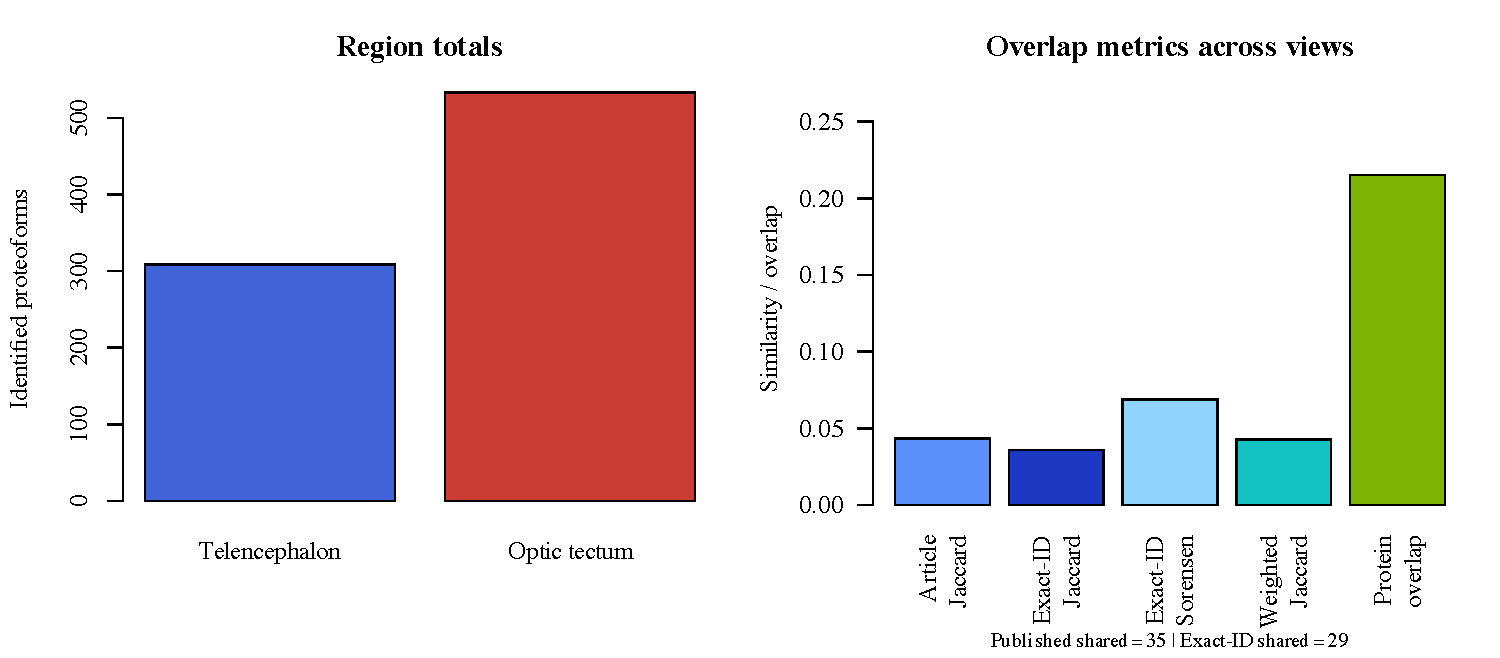
\includegraphics[width=0.97\linewidth]{../figures/fig1_region_overview.pdf}
    \caption{Regional totals and overlap metrics. The exact-ID source-table view is slightly stricter than the article aggregate, but both place telencephalon and optic tectum in the same low-overlap regime.}
    \label{fig:region-overview}
\end{figure}

\subsection{The source paper's biological interpretation becomes much stronger when expressed as an alignment problem}

A second substantive result is that this regional split is biologically organized in the expected direction. The curated marker panel is highly concentrated in the expected region. Telencephalon-associated markers contribute 23 matched counts and only 2 spillover counts, for an axis-level alignment fraction of 0.9200. Optic-tectum-associated markers contribute 102 matched counts and 1 spillover count, for an alignment fraction of 0.9903. Across the whole panel, the observed matched-region fraction is 0.9766. A naive baseline built only from the panel's own 25-versus-103 telencephalon/optic-tectum prevalence would predict 0.6904, so the observed alignment still exceeds that baseline by 0.2861. This matters because optic tectum contributes the larger raw proteoform total in the source study; the alignment result is therefore not just a restatement of optic-tectum abundance.

When those counts are written as a $2\times2$ table, the odds ratio is 1173 with an approximate 95\% confidence interval from 102.0 to 13{,}495.1, and the one-sided exact p-value is 5.12$\times10^{-22}$. The interval is necessarily wide because the off-diagonal cells are sparse, but even its lower bound still corresponds to a very large effect. The exact test is helpful, but the more intuitive story is the effect size: both functional axes sit far above the baseline expected from regional prevalence alone. The family-size-preserving randomization test makes the same point in a way that does not depend on asymptotic odds-ratio logic. Under 200{,}000 randomizations that preserved the nine family sizes and the global 25-versus-103 telencephalon/optic-tectum label totals, the null mean was only 88.4 matched counts and the 95th percentile was 95; none of those draws reached the observed 125 matched counts, giving a one-sided Monte Carlo upper bound of $5\times10^{-6}$.

These numbers do not imply that the entire proteome has been functionally classified. They mean something narrower and more useful: the particular marker proteoforms that the source article called biologically meaningful are overwhelmingly concentrated in the region whose known function they should support. That is the sense in which this paper turns a qualitative regional intuition into an explicit biological statement.

The count-based result is not hiding a family-composition problem. All 9 curated marker groups favor their expected region, the mean family-level matched share is 0.9826, the weakest family-level matched share is still 0.8750, and the corresponding one-sided sign-style probability under a 50:50 null is 0.001953. The conclusion is also stable across two stronger robustness moves that were not available in earlier versions of this paper. First, collapsing the curated panel to unique proteins still yields 28 matched proteins versus only 2 spillover proteins, for an alignment fraction of 0.9333, an odds ratio of 147.0, and a one-sided exact p-value of 3.02$\times10^{-5}$. A protein-collapsed family-size-preserving randomization tells the same story: the null mean is only 18.27 matched proteins, the 95th percentile is 22, and none of 200{,}000 draws reaches the observed 28 (Monte Carlo upper bound $=4\times10^{-5}$). Second, weighting the same panel by mean duplicate intensity yields a matched-region fraction of 0.9966, showing that the count-level result is not being driven by many weak spillover signals.

\begin{figure}[t]
    \centering
    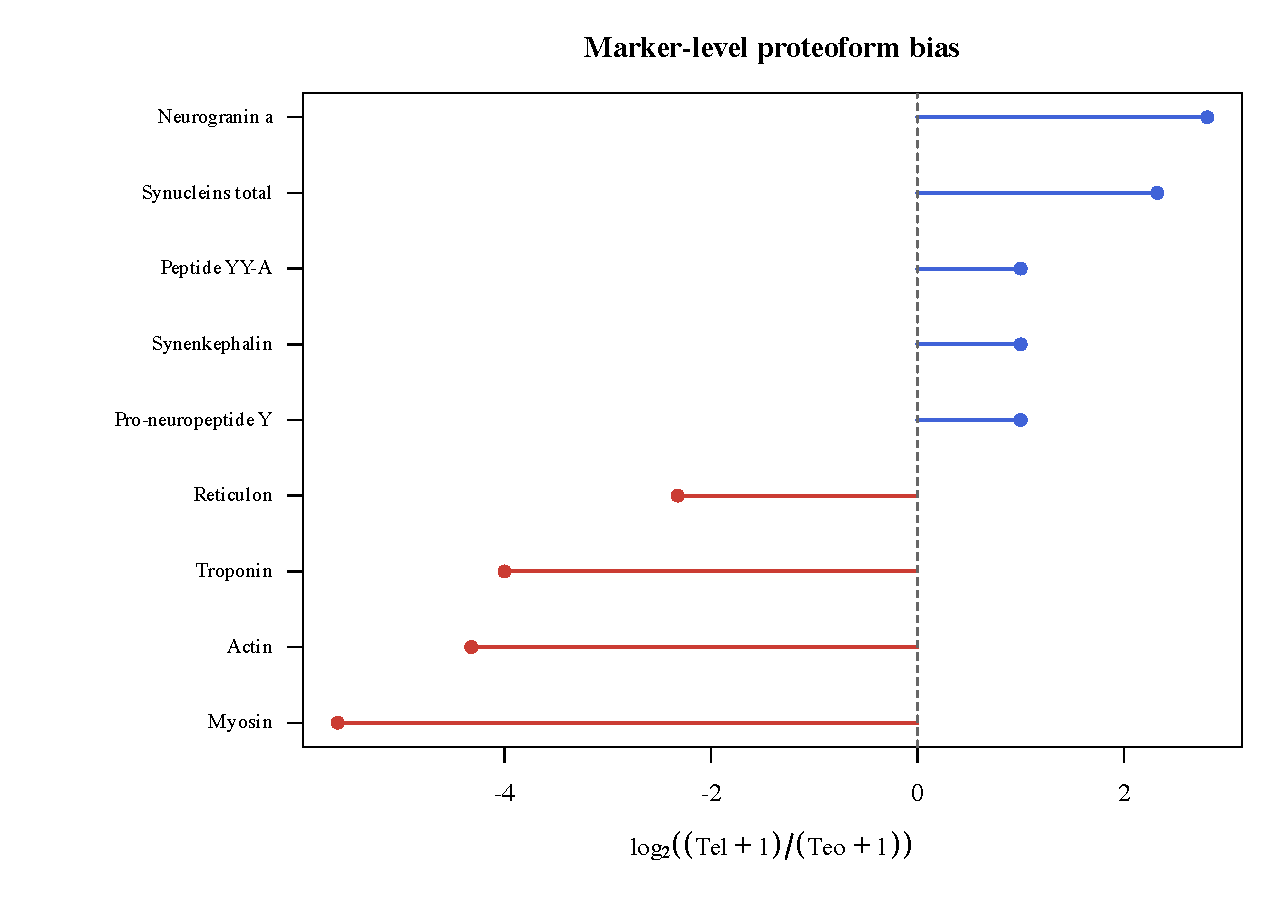
\includegraphics[width=0.90\linewidth]{../figures/fig2_marker_bias.pdf}
    \caption{Marker-level proteoform bias. Positive values favor telencephalon and negative values favor optic tectum.}
    \label{fig:marker-bias}
\end{figure}

\begin{figure}[t]
    \centering
    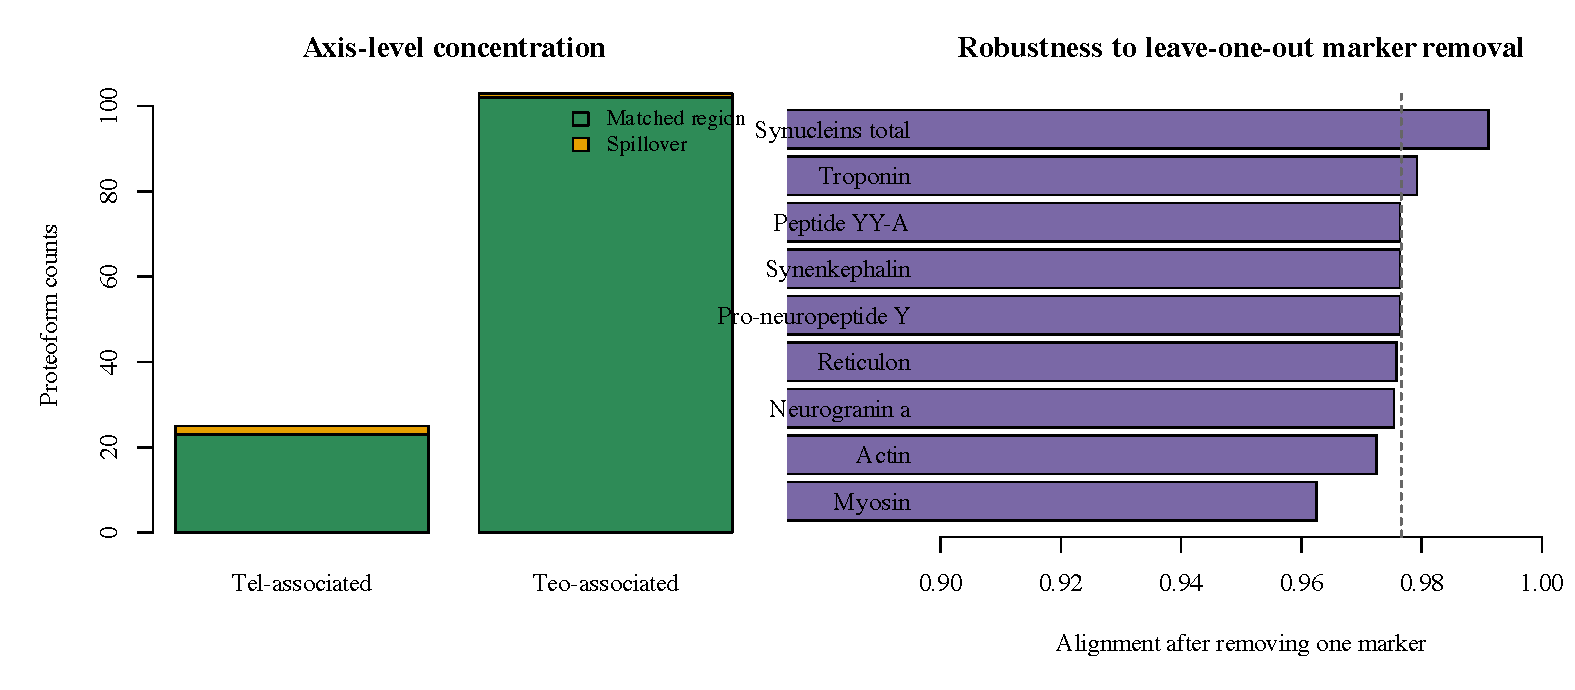
\includegraphics[width=0.97\linewidth]{../figures/fig3_axis_alignment.pdf}
    \caption{Axis-level concentration and robustness summaries. The overall alignment signal remains high after leave-one-out perturbation, after excluding motor families, after collapsing to proteins, and after weighting by mean duplicate intensity.}
    \label{fig:axis-alignment}
\end{figure}

\begin{table}[t]
\centering
\caption{Curated marker families used in the axis-alignment analysis. The released source tables now expose exact accession+proteoform members for each family in the local marker-membership file, but the biological framing still follows the source paper's named marker groups.}
\label{tab:markers}
\begin{tabular}{lrrl}
\toprule
Marker group & Tel & Teo & Interpretation \\
\midrule
Pro-neuropeptide Y & 1 & 0 & feeding-related neuropeptide signaling \\
Synenkephalin & 1 & 0 & affective signaling \\
Peptide YY-A & 1 & 0 & peptide hormone signaling \\
Neurogranin a & 6 & 0 & memory-linked synaptic signaling \\
Synucleins total & 14 & 2 & synaptic and mnemonic family \\
Reticulon & 0 & 4 & retinotectal organization \\
Myosin & 0 & 48 & motor machinery \\
Actin & 0 & 19 & cytoskeletal movement \\
Troponin & 1 & 31 & contraction-linked regulation \\
\bottomrule
\end{tabular}
\end{table}

\begin{table}[t]
\centering
\caption{Axis-level alignment compared with the naive baseline implied by regional prevalence.}
\label{tab:axisstats}
\begin{tabular}{lrrrr}
\toprule
Functional axis & Observed & Wilson 95\% CI & Baseline & Lift \\
\midrule
Telencephalon-associated & 0.9200 & 0.7503--0.9778 & 0.1875 & 0.7325 \\
Optic-tectum-associated & 0.9903 & 0.9470--0.9983 & 0.8125 & 0.1778 \\
\bottomrule
\end{tabular}
\end{table}

The leave-one-out analysis in Figure~\ref{fig:axis-alignment} also stays strong numerically: the matched-region fraction ranges only from 0.9625 to 0.9911 after removing any single marker family. The worst case comes from removing the large myosin group, yet even that stress test remains far above the naive prevalence baseline.

A second set of stress tests addresses the most obvious reviewer-style objections. If one, two, or three matched counts on each axis are pessimistically reassigned to spillover, the overall alignment fraction remains 0.9609, 0.9453, and 0.9297, respectively, while the odds ratio remains between 99.0 and 370.3. If the motor-associated myosin, actin, and troponin families are removed entirely to probe whether the optic-tectum signal is mainly a local contamination story, the remaining panel still aligns at 0.9310 with a Haldane-corrected odds ratio of 84.6. A lightweight composition guardrail points in the same direction: the released tables contain only 2 optic-tectum glial-support sentinels (GFAP and S100B) but 23 telencephalon myelin sentinels (MBPA/B) versus 3 in optic tectum. These checks do not eliminate missingness or purity concerns, but they show that the main regional-function signal is not being carried by a single fragile bookkeeping choice.

The review also asked for an independently curated panel that was not inherited from the source paper's own prose. Using adult zebrafish myelin markers from the zebrafish CNS myelin literature (PLP1b, MBPa, MBPb, MPZ/P0) together with adult optic-tectum radial-glia markers from the tectal precursor literature (GFAP, FABP7a, S100B) yields the same qualitative result. This independent panel contributes 32 matched counts and only 3 spillover counts, for an alignment fraction of 0.9143, an odds ratio of 73.3, and a one-sided exact p-value of $6.68\times10^{-4}$. After collapsing to proteins, the panel still aligns at 0.8750 with an odds ratio of 37.8 and $p = 0.00824$. The panel is smaller and more composition-oriented than the source paper's functional families, so it should not be read as a substitute for them. What it does show is that the regional separation signal is not resting entirely on the source paper's own choice of biologically favored markers.

\begin{table}[t]
\centering
\caption{Sensitivity checks requested by the external review. The motor-family exclusion uses a Haldane correction because one spillover cell is zero after exclusion.}
\label{tab:sensitivity}
\begin{tabular}{lrrr}
\toprule
Scenario & Alignment & Odds ratio & One-sided $p$ \\
\midrule
Observed panel & 0.9766 & 1173.0 & 5.12$\times10^{-22}$ \\
Shift 1 matched count per axis & 0.9609 & 370.3 & 2.01$\times10^{-19}$ \\
Shift 2 matched counts per axis & 0.9453 & 175.0 & 3.73$\times10^{-17}$ \\
Shift 3 matched counts per axis & 0.9297 & 99.0 & 3.93$\times10^{-15}$ \\
Exclude myosin, actin, troponin & 0.9310 & 84.6 & 6.32$\times10^{-4}$ \\
\bottomrule
\end{tabular}
\end{table}

\subsection{The pilot is PTM-rich and technically sensitive enough to justify proteoform-level interpretation}

The PTM follow-up contributes a third kind of knowledge, namely a disciplined negative result about what the public evidence does and does not support. The source article reports 807 identified proteoforms in total, of which 358 carry mass shifts and 211 are N-terminally acetylated. That means 44.36\% of the detected proteoforms belong to the modified subset and 58.94\% of the modified subset is N-terminally acetylated. These totals reinforce a simple point: the dataset is not just a protein list wearing different formatting. A large part of the biological signal lives at the proteoform level.

The source tables let us connect that PTM layer back to the regional marker analysis, but the reviewer-driven follow-up substantially changes how strongly we should read it. In the raw matched-marker counts, 14 of 23 telencephalon-matched proteoforms are N-terminally acetylated (0.6087), compared with only 16 of 102 optic-tectum-matched proteoforms (0.1569), for an unadjusted odds ratio of 8.36 and a one-sided exact p-value of $2.53\times10^{-5}$. That acetylation result remains significant after Holm correction across the two PTM screens in this paper (adjusted $p = 5.05\times10^{-5}$). By contrast, an exploratory ``other mass shift'' bucket shows 5/23 telencephalon-matched proteoforms and 20/102 optic-tectum-matched proteoforms, with no directional enrichment ($p = 0.508$).

The new detectability checks make the acetylation claim much more fragile. Among the acetylated matched-marker subsets, telencephalon rows are heavier (mean precursor mass 10{,}824.6 versus 6202.4; permutation $p = 3.05\times10^{-4}$), longer (mean residue span 106.1 versus 55.8; $p = 7.5\times10^{-5}$), and closer to the protein N terminus (mean first residue 1.0 versus 1.94; $p = 5\times10^{-6}$), while the mean duplicate intensity does not differ materially ($p = 0.417$). Once acetylation is rechecked in a coarse logistic sensitivity that adjusts for log precursor mass, span length, and first-residue position, the odds ratio falls to 2.94 with a 95\% confidence interval of 0.70--12.30 ($p = 0.140$). Restricting the analysis to matched-marker rows whose first residue lies at or within two positions of the N terminus removes the enrichment entirely (odds ratio 0.88, one-sided $p = 0.714$). The right reading is therefore no longer ``robust acetylation enrichment.'' It is that the public tables contain an interesting acetylation asymmetry, but that asymmetry is not stable once the available geometry and coverage proxies are taken seriously.

The technical-sensitivity numbers are also useful. The duplicate analyses yielded means of 232 proteoforms for telencephalon and 356 for optic tectum, corresponding to recovery fractions of 0.7508 and 0.6680 relative to the regional totals. The same released tables expose the incidence counts needed for Chao2 lower bounds: $q_1=154$, $q_2=155$ for telencephalon and $q_1=355$, $q_2=178$ for optic tectum. The single-run high-water mark was 418 proteoforms from an injected amount corresponding to roughly 250 cells in the source paper, or about 1.672 proteoforms per estimated sampled cell. That does not eliminate the pilot-study caveat, but it does explain why the study was able to expose biologically legible regional structure from very small samples while still leaving room for unseen-overlap sensitivity analyses.

\begin{table}[t]
\centering
\caption{Technical sensitivity values reported in the source study and extended with duplicate-incidence counts from the released source tables.}
\label{tab:technical}
\begin{tabular}{lrrrrrr}
\toprule
Region & Duplicate mean & Duplicate SD & CV & Recovery & $q_1$ & Chao2 lower bound \\
\midrule
Telencephalon & 232 & 28 & 0.1207 & 0.7508 & 154 & 385.5 \\
Optic tectum & 356 & 88 & 0.2472 & 0.6680 & 355 & 887.0 \\
\bottomrule
\end{tabular}
\end{table}

\begin{figure}[t]
    \centering
    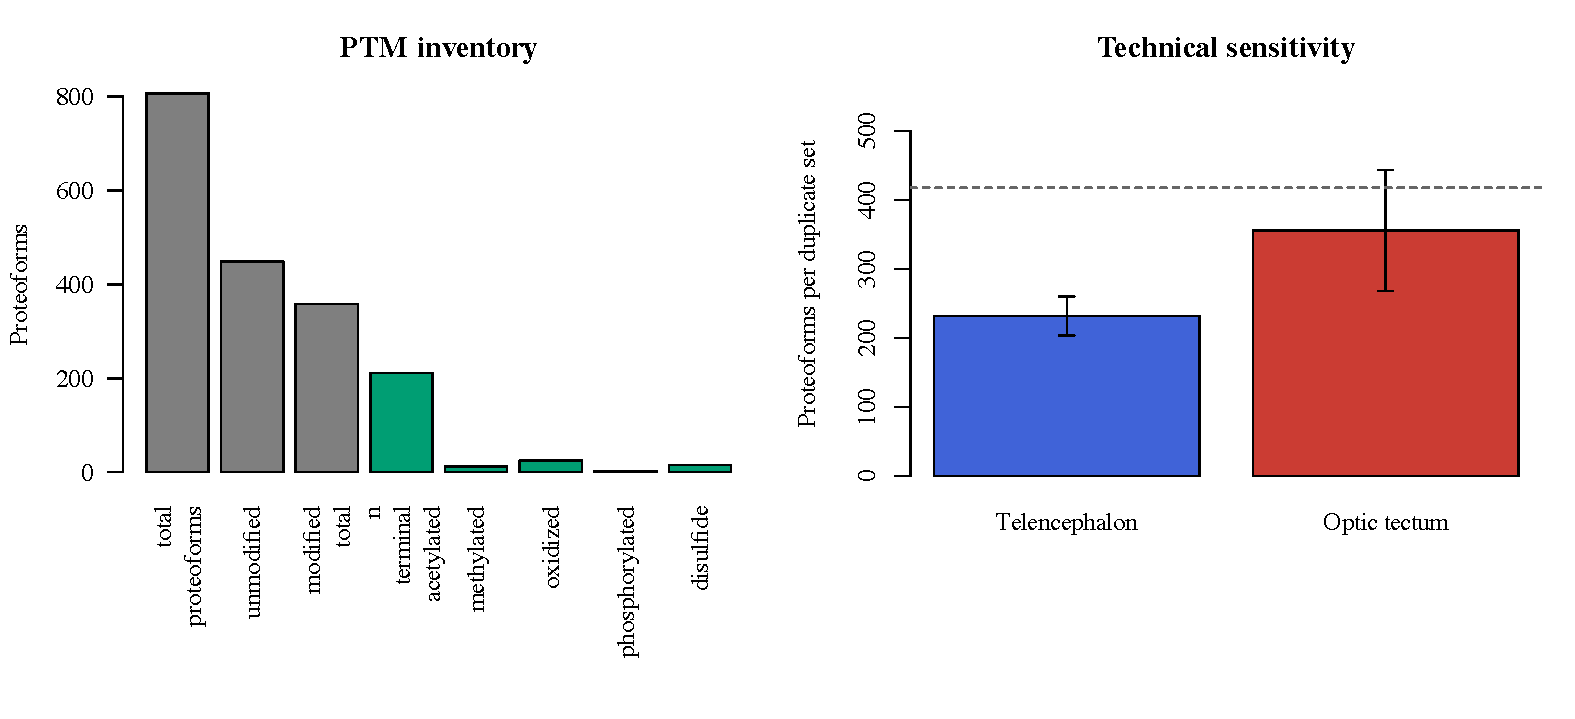
\includegraphics[width=0.97\linewidth]{../figures/fig4_ptm_and_sensitivity.pdf}
    \caption{PTM and missingness-sensitive follow-up analyses. Left: N-terminal acetylation is much more common in the telencephalon-matched marker subset than in the optic-tectum-matched subset. Right: duplicate-informed Chao2 sensitivity changes the exact-ID Jaccard modestly, but it never turns the regional split into a high-overlap regime.}
    \label{fig:ptm-sensitivity}
\end{figure}
